记 $\hat\kappa$ 为参考空间 $(\hat x_1,\hat x_2)$ 中的参考单位正方形
$[0,1]\times[0,1]$, 其顶点如 Figure
\ref{fig:appendix-quadrilateral-reference-square} 所示记为
$\hat a_j$, $1\leq j\leq4$.
按照该图中的记号, 对每个顶点为 $a_j$ 的凸四边形 $\kappa$,
恰有一个可逆映射 $F_\kappa\in Q_1^2$ 把 $\hat\kappa$ 映到
$\kappa$, 并满足
\[
F_\kappa(\hat a_j)=a_j,
\qquad
1\leq j\leq4.
\]

\begin{figure}[htbp]
\centering
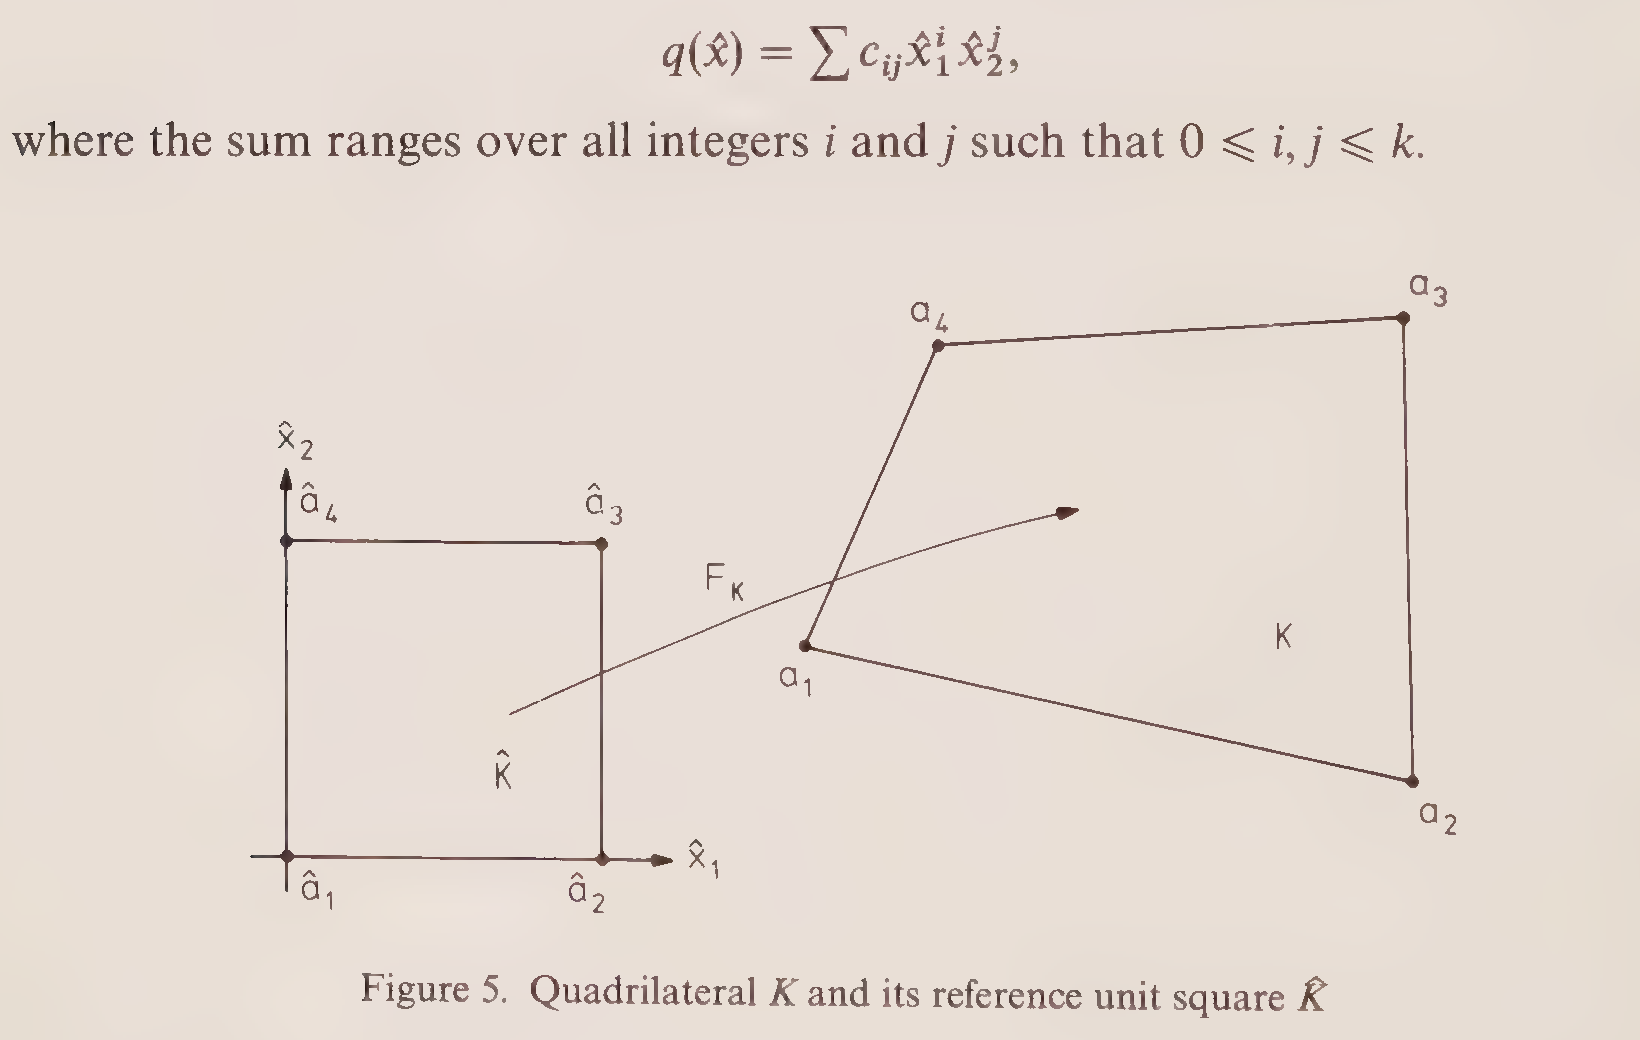
\includegraphics[width=.80\linewidth]{figures/appendix-figure-5.png}
\caption{四边形 $\kappa$ 及其参考单位正方形 $\hat\kappa$.}
\label{fig:appendix-quadrilateral-reference-square}
\end{figure}

\MathBookSourcePage{119}
记 $S_i$ 为 $\kappa$ 中以 $a_{i-1}$, $a_i$, $a_{i+1}$ 为顶点的
子三角形(其中 $a_0$ 与 $a_4$ 相同).
注意, 除非 $\kappa$ 是平行四边形, 否则映射 $F_\kappa$ 不是仿射的;
但它仍把 $\hat\kappa$ 的各边映到 $\kappa$ 的对应边上,
而且 $F_\kappa$ 在 $\hat\kappa$ 各边上的限制确实是仿射的.

对每个 $\hat x$, 令
\[
DF_\kappa(\hat x)
=
\left[
\frac{\partial F_i(\hat x)}{\partial\hat x_j}
\right]_{i,j}
\in
\mathcal{L}(\mathbb{R}^2;\mathbb{R}^2)
\]
表示 $F_\kappa$ 在 $\hat x$ 处的导数, 并赋予范数
\[
\|DF_\kappa\|_{\infty,\hat\kappa}
=
\sup_{\hat x\in\hat\kappa}\|DF_\kappa(\hat x)\|,
\]
其中照常用 $\|\cdot\|$ 表示从属 Euclidean 范数.
令 $J_F$ 表示 $F_\kappa$ 的 Jacobian, 即
\[
J_F(\hat x)=\det(DF_\kappa(\hat x)).
\]
若 $F_\kappa^{-1}$ 表示 $F_\kappa$ 的逆, 其 Jacobian 为
$J_{F^{-1}}$, 则
\begin{equation}\label{eq:appendix-quadrilateral-inverse-derivative-jacobian}
D(F_\kappa^{-1})\circ F_\kappa
=
(DF_\kappa^T)^{-1},
\qquad
J_{F^{-1}}\circ F_\kappa
=
1/J_F.
\end{equation}
再次注意, 当 $F_\kappa$ 为仿射映射时,
$DF_\kappa=B_\kappa$,
$D(F_\kappa^{-1})=(B_\kappa^T)^{-1}$,
$J_F=\det(B_\kappa)$.
当然, 由于 $J_F$ 不是常数, 简单关系
\eqref{eq:appendix-simplex-determinant-measure} 在这里不成立;
但直接计算表明 $J_F\in P_1$, 因而其极值在 $\hat\kappa$ 的顶点处取得.
于是容易验证
\begin{equation}\label{eq:appendix-quadrilateral-jacobian-extrema}
\left\{
\begin{aligned}
\max_{\hat x\in\hat\kappa}J_F(\hat x)
&=
2\max_{1\leq i\leq4}\operatorname{meas}(S_i),\\
\min_{\hat x\in\hat\kappa}J_F(\hat x)
&=
2\min_{1\leq i\leq4}\operatorname{meas}(S_i),
\end{aligned}
\right.
\end{equation}
并注意到
\[
J_F(\hat x)\geq0,
\]
因为 $\kappa$ 是凸的. 此外,
\[
J_F(1/2,1/2)=\operatorname{meas}(\kappa).
\]
因此, 由 \eqref{eq:appendix-quadrilateral-inverse-derivative-jacobian}
和 \eqref{eq:appendix-quadrilateral-jacobian-extrema} 可见,
描述 $\kappa$ 几何的一个方便的参数选择是
\[
h_\kappa=\text{$\kappa$ 的直径},
\]
\[
\rho_\kappa
=
2\min_{1\leq i\leq4}
\{\,\text{$S_i$ 中内切圆的直径}\,\}.
\]
这个选择给出下列上界:
\begin{equation}\label{eq:appendix-quadrilateral-map-bounds}
\left\{
\begin{aligned}
\|DF_\kappa\|_{\infty,\hat\kappa}
&\leq C_1h_\kappa,
&\qquad
\|J_F\|_{\infty,\hat\kappa}
&\leq C_2h_\kappa^2,\\
\|DF_\kappa^{-1}\|_{\infty,\kappa}
&\leq C_3h_\kappa/\rho_\kappa^2,
&
\|J_{F^{-1}}\|_{\infty,\kappa}
&\leq C_4/\rho_\kappa^2,
\end{aligned}
\right.
\end{equation}
其中所有常数都与 $\kappa$ 的几何无关.

三角剖分 $\mathcal{T}_h$ 仍使用相同概念, 不同之处只是它由凸四边形
而非三角形组成. 对上述参数, 我们保留 Definition
\ref{def:appendix-regular-triangulation} 中正则和一致正则三角剖分的定义.
注意, 三角剖分的正则性保证 $\kappa$ 的任何子三角形都具有非零测度,
即 $\kappa$ 不会退化成三角形.

\MathBookSourcePage{120}
下面转向有限元空间. 由四边形的几何可知,
这里的基函数不是 $P_k$ 中的多项式, 而是 $Q_k$ 中多项式的像.
更确切地, 对每个整数 $k\geq0$ 和 $\mathcal{T}_h$ 的每个单元
$\kappa$, 引入有限维空间
\begin{equation}\label{eq:appendix-quadrilateral-local-space}
Q_k(\kappa)
=
\{\,q=\hat q\circ F_\kappa^{-1};\ \hat q\in Q_k\,\}.
\end{equation}
注意 $Q_k(\kappa)\subset\mathcal{C}^\infty(\kappa)$,
但除非 $\kappa$ 是平行四边形, $Q_k(\kappa)$ 并非多项式空间.
为了研究这种空间中的逼近误差, 必须略微修改 Theorem
\ref{thm:appendix-bramble-hilbert-general} 及其推论的陈述.
这可通过改变半范数做到. 对每个整数 $k\geq0$ 和实数 $p>0$, 令
\begin{equation}\label{eq:appendix-directional-seminorm}
[v]_{k,p,\Omega}
=
\left(
\left\|\frac{\partial^kv}{\partial x_1^k}\right\|_{0,p,\Omega}^p
+
\left\|\frac{\partial^kv}{\partial x_2^k}\right\|_{0,p,\Omega}^p
\right)^{1/p}.
\end{equation}
显然,
$[\cdot]_{0,p,\Omega}=\|\cdot\|_{0,p,\Omega}$,
$[\cdot]_{1,p,\Omega}=|\cdot|_{1,p,\Omega}$.
此外, 这个半范数具有 Aronszajn \& Smith 证明的下列重要性质
(参见 Smith [74]).

\setcounter{statement}{7}
\begin{Lemma}\label{lem:appendix-directional-seminorm-equivalence}
设 $\Omega$ 是 $\mathbb{R}^2$ 中具有 Lipschitz 连续边界的有界区域.
对每个整数 $k\geq0$ 和实数 $p>0$, 存在正常数 $C$, 使得
\begin{equation}\label{eq:appendix-directional-seminorm-equivalence}
\|v\|_{k,p,\Omega}
\leq
C\{\,\|v\|_{0,p,\Omega}+[v]_{k,p,\Omega}\,\}
\qquad
\forall v\in W^{k,p}(\Omega).
\end{equation}
\end{Lemma}

现在, Theorem \ref{thm:appendix-bramble-hilbert-general}
及其第一个推论有如下对应结果.

\setcounter{statement}{2}
\begin{Theorem}\label{thm:appendix-quadrilateral-bramble-hilbert}
设 $k\geq0$, $m\geq0$ 为整数, $p\geq1$, $q\geq1$ 为实数, 且
\[
W^{k+1,p}(\hat\kappa)\hookrightarrow W^{m,q}(\hat\kappa).
\]
设
$\hat\pi\in\mathcal{L}(W^{k+1,p}(\hat\kappa);W^{m,q}(\hat\kappa))$
满足
\[
\hat\pi t=t
\qquad
\forall t\in Q_k.
\]
则存在一个仅依赖于 $k$, $m$, $p$, $q$, $\hat\kappa$ 和 $\hat\pi$
的正常数 $\hat C$, 使得
\begin{equation}\label{eq:appendix-quadrilateral-bramble-hilbert}
|\hat v-\hat\pi\hat v|_{m,q,\hat\kappa}
\leq
\hat C[\hat v]_{k+1,p,\hat\kappa}
\qquad
\forall\hat v\in W^{k+1,p}(\hat\kappa).
\end{equation}
\end{Theorem}

为了估计 $Q_k(\kappa)$ 中的插值误差, 必须用 $\hat v$ 估计
$|v|_{m,q,\kappa}$, 并用 $v$ 估计
$[\hat v]_{k+1,p,\hat\kappa}$. 这是下一个 Lemma 的内容
(与 Lemma \ref{lem:appendix-simplex-change-of-variables} 比较).
证明所需材料可见 Cartan [17].

\setcounter{statement}{8}
\begin{Lemma}\label{lem:appendix-quadrilateral-change-of-variables}
设 $\kappa$ 是凸四边形. 对每个整数 $m\geq0$ 和实数
$p\in[1,\infty]$, 存在与 $\kappa$ 的几何无关的正常数
$C_1$, $C_2$, $C_3$, 使得对所有 $v\in W^{m,p}(\kappa)$ 有
\begin{equation}\label{eq:appendix-quadrilateral-change-physical}
\left\{
\begin{aligned}
|v|_{0,p,\kappa}
&\leq
C_1h_\kappa^{2/p}|\hat v|_{0,p,\hat\kappa},\\
|v|_{m,p,\kappa}
&\leq
C_2(h_\kappa/\rho_\kappa)^{3m-2}
\frac{h_\kappa^{2/p}}{\rho_\kappa^m}
\left\{\sum_{i=1}^m|\hat v|_{i,p,\hat\kappa}^p\right\}^{1/p},
\qquad m\geq1,
\end{aligned}
\right.
\end{equation}
以及
\begin{equation}\label{eq:appendix-quadrilateral-change-reference}
[\hat v]_{m,p,\hat\kappa}
\leq
C_3\frac{h_\kappa^m}{\rho_\kappa^{2/p}}
|v|_{m,p,\kappa},
\qquad
m\geq0.
\end{equation}
\end{Lemma}

\MathBookSourcePage{121}
由此得到 Corollary
\ref{cor:appendix-abstract-interpolation-physical} 的下列对应结果
(与 Remark \ref{rem:appendix-local-interpolation-estimate} 比较).

\setcounter{statement}{4}
\begin{Corollary}\label{cor:appendix-quadrilateral-interpolation-error}
设 $\kappa$ 是凸四边形, $k$, $m$, $p$, $q$ 和 $\hat\pi$ 如
Theorem \ref{thm:appendix-quadrilateral-bramble-hilbert} 中所述.
定义算子
$\pi\in\mathcal{L}(W^{k+1,p}(\kappa);W^{m,q}(\kappa))$ 为
\[
\widehat{\pi v}=\hat\pi\hat v.
\]
则存在与 $\kappa$ 的几何无关的正常数 $C$, 使得
\begin{equation}\label{eq:appendix-quadrilateral-interpolation-error}
\left\{
\begin{aligned}
|v-\pi v|_{0,q,\kappa}
&\leq
C\sigma_\kappa^{2/p}
h_\kappa^{k+1+2/q-2/p}
|v|_{k+1,p,\kappa},\\
|v-\pi v|_{m,q,\kappa}
&\leq
C\sigma_\kappa^{4m-2+2/p}
h_\kappa^{k+1-m+2/q-2/p}
|v|_{k+1,p,\kappa},
&&m\geq1,\\
&&&\forall v\in W^{k+1,p}(\kappa).
\end{aligned}
\right.
\end{equation}
当 $\kappa$ 属于正则三角剖分 $\mathcal{T}_h$ 时, 这两个不等式化为
\begin{equation}\label{eq:appendix-quadrilateral-interpolation-error-regular}
|v-\pi v|_{m,q,\kappa}
\leq
Ch^{k+1-m+2/q-2/p}|v|_{k+1,p,\kappa}.
\end{equation}
\end{Corollary}

\setcounter{statement}{2}
\begin{Remark}\label{rem:appendix-quadrilateral-cross-derivatives}
对所有 $m\geq2$, 关于复合函数求导的一个简单练习表明,
与 $[\hat v]_{m,p,\hat\kappa}$ 不同,
完整半范数 $|\hat v|_{m,p,\hat\kappa}$ 用
$\|v\|_{m,p,\kappa}$ 表示的上界非常差.
问题来自交叉导数
$\partial^m\hat v/(\partial\hat x_1^i\partial\hat x_2^{m-i})$,
$1\leq i\leq m-1$, 因为它们特别含有因子
$\partial^2F_\kappa/(\partial\hat x_1\partial\hat x_2)$,
而不是形如
$(\partial F_\kappa/\partial\hat x_k)
(\partial F_\kappa/\partial\hat x_l)$ 的乘积.
除非 $\kappa$ 接近平行四边形,
$\partial^2F_\kappa/(\partial\hat x_1\partial\hat x_2)$
仅为 $h_\kappa$ 阶, 而
$(\partial F_\kappa/\partial\hat x_k)
(\partial F_\kappa/\partial\hat x_l)$ 为 $h_\kappa^2$ 阶.
这就是半范数 $[\cdot]_{m,p,\Omega}$ 在推导四边形有限元的精确误差估计时
起关键作用的原因.
\end{Remark}

\setcounter{statement}{3}
\begin{Remark}\label{rem:appendix-quadrilateral-regularity-exponent}
注意, \eqref{eq:appendix-quadrilateral-interpolation-error}
中的正则性因子 $\sigma_\kappa$ 的指数远高于
\eqref{eq:appendix-local-interpolation-estimate} 中的指数.
这是因为变换 $F_\kappa$ 不是仿射的.
\end{Remark}

与上一节相同, 固定整数 $k\geq1$, 并引入类似的有限元空间
\[
\Theta_h
=
\{\,\theta_h\in\mathcal{C}^0(\bar\Omega);
\ \theta_h|_\kappa\in Q_k(\kappa)
\quad\forall\kappa\in\mathcal{T}_h\,\},
\]
\[
\Phi_h=\Theta_h\cap H_0^1(\Omega).
\]
我们首先在 $\hat\kappa$ 的 $k$ 阶主格点(参见 Figure
\ref{fig:appendix-principal-lattice-order-three})上插值函数值,
以得到 $I_h$ 的对应算子:
\[
\Sigma_{\hat\kappa}
=
\{\,(i/k,j/k);\ 0\leq i,j\leq k\,\}.
\]
即对每个 $\hat v\in\mathcal{C}^0(\hat\kappa)$, 令
\begin{equation}\label{eq:appendix-quadrilateral-lagrange-reference}
\hat I\hat v\in Q_k,
\qquad
\hat I\hat v(\hat x)=\hat v(\hat x)
\quad
\forall\hat x\in\Sigma_{\hat\kappa}.
\end{equation}

\MathBookSourcePage{122}
若 $\mathcal{T}_h$ 正则, 在 $\mathcal{T}_h$ 的每个 $\kappa$ 上由
\[
\widehat{I_hv}=\hat I\hat v
\qquad
\forall v\in\mathcal{C}^0(\bar\Omega)
\]
定义的插值算子 $I_h$ 满足 Lemma
\ref{lem:appendix-lagrange-interpolation} 的结论, 即
\begin{equation}\label{eq:appendix-quadrilateral-lagrange-error-wsp}
\begin{aligned}
|v-I_hv|_{m,p,\Omega}
&\leq
Ch^{s+1-m}|v|_{s+1,p,\Omega}
&&\forall v\in W^{s+1,p}(\Omega),\\
&\forall m\in\mathbb{N},\quad
\forall s,p\in\mathbb{R}
\text{ with }p>1,\\
&\qquad
0\leq m\leq s+1,\quad
1\leq s\leq k,
\end{aligned}
\end{equation}
以及
\begin{equation}\label{eq:appendix-quadrilateral-lagrange-error-w1q}
|v-I_hv|_{m,q,\Omega}
\leq
Ch^{1-m}|v|_{1,q,\Omega}
\qquad
\forall v\in W^{1,q}(\Omega),
\quad q>2,
\quad m=0,1.
\end{equation}

类似地, 对 $p>1$, 在 $W^{2,p}(\hat\kappa)$ 上定义插值算子
$\widetilde I_{\hat\kappa}$:
\[
\widetilde I_{\hat\kappa}\hat v\in Q_k,
\]
\[
\widetilde I_{\hat\kappa}\hat v(\hat a_i)=\hat v(\hat a_i),
\qquad
1\leq i\leq4,
\]
并且当 $k\geq2$ 时,
\[
\left\{
\begin{aligned}
\int_{\hat\kappa'}
(\widetilde I_{\hat\kappa}\hat v-\hat v)f\,\mathrm{d}\hat s
&=0
&&\forall f\in P_{k-2}(\hat\kappa'),
\quad\text{对 $\hat\kappa$ 的每条边 $\hat\kappa'$},\\
\int_{\hat\kappa}
(\widetilde I_{\hat\kappa}\hat v-\hat v)f\,\mathrm{d}\hat x
&=0
&&\forall f\in Q_{k-2}(\hat\kappa).
\end{aligned}
\right.
\]
沿 Lemma \ref{lem:appendix-moment-interpolant-local} 的思路容易证明,
这个线性方程组唯一地定义了 $\widetilde I_{\hat\kappa}$.
于是, 若 $\mathcal{T}_h$ 正则, 在 $\mathcal{T}_h$ 的每个
$\kappa$ 上由
\[
\widehat{\widetilde I_hv}
=
\widetilde I_{\hat\kappa}\hat v
\qquad
\forall v\in W^{2,p}(\Omega),
\quad p>1,
\]
定义的算子 $\widetilde I_h$ 满足 Lemma
\ref{lem:appendix-moment-interpolant-global} 的陈述.

同样, 投影 $P_h$ 和 $\dot P_h$ 可以推广到四边形情形,
并且可以证明它们具有与三角形情形相同的性质.
类似地, 在 $\hat\kappa$ 上由
\begin{equation}\label{eq:appendix-quadrilateral-l2-projection}
\left\{
\begin{aligned}
\hat\rho\hat v&\in Q_k,\\
\int_{\hat\kappa}(\hat\rho\hat v-\hat v)f\,\mathrm{d}\hat x&=0
&&\forall f\in Q_k,
\end{aligned}
\right.
\quad\text{on }\hat\kappa,
\qquad
\widehat{\rho_hv}=\hat\rho\hat v
\quad
\forall\kappa\in\mathcal{T}_h,
\end{equation}
定义的 $L^2$ 投影 $\rho_h$ 在三角剖分正则的条件下满足
Lemma \ref{lem:appendix-local-l2-projection-error} 的陈述.

最后, Lemma \ref{lem:appendix-local-inverse-inequality} 和 Corollary
\ref{cor:appendix-global-inverse-gradient} 对四边形有限元仍然成立;
而一般而言, Lemma \ref{lem:appendix-global-inverse-same-order}
在这里仅当 $m\leq1$ 时成立. 不过, $m$ 的这两个取值已足够用于后续应用.
